\chapter{Semantische Analyse} \label{chap:semantic}

Die semantische Analyse ist notwendig, da ein syntaktisch korrektes Programm logische Fehler beinhalten kann. Ein Beispiel dafür ist in \cref{lst:semantic-error} zu sehen. Darin wird eine Variable gelesen, bevor diese definiert wurde. Ein weiterer Fehler wäre es beispielsweise eine Funktion mit zu wenigen Parametern aufzurufen. Die Aufgabe der semantischen Analyse ist es, den erzeugten \ac{ast} zu durchlaufen und dabei die einzelnen Knoten auf solche Fehler zu prüfen.

\begin{lstlisting}[language=c, caption=Beispiel für einen semantischen Fehler, label={lst:semantic-error}]
	var r0 := r1;
	var r1 := 2;
\end{lstlisting}

\section{Abbilden auf eine Datenstruktur}
Um logische Fehler zu erkennen, bietet es sich an, eine eigene Datenstruktur zu entwerfen, welche das Programm abbildet und beim Durchlaufen des \ac{ast} diese Datenstruktur zu füllen. So kann beispielsweise bei einem Funktionsaufruf in der Datenstruktur nachgesehen werden, ob die entsprechende Funktion bereits deklariert wurde oder noch nicht. Ein weiterer Vorteil davon, eine solche Datenstruktur zu definieren, ist es, dass nach dem erfolgreichen Befüllen die Datenstruktur ausschließlich ein syntaktisch und semantisch korrektes Programm abbildet. Es wäre denkbar, die erzeugte Datenstruktur in einem nächsten Schritt anhand der gesammelten Daten zu optimieren und beispielsweise unbenutzte Funktionen zu entfernen, dies geschieht im aktuellen Stand der Arbeit nicht.

In \cref{pic:Semantic-Struct} ist zu sehen, wie ein While-Programm auf eine Java-Klasse abgebildet wird. Knoten aus dem \ac{ast}, welche nicht relevant für die semantische Überprüfung oder die Codegenerierung sind, wie beispielsweise Semikolon oder Klammern werden nicht in die Datenstruktur mit aufgenommen, sondern ausschließlich Daten wie Variablennamen, Werte einer Zuweisung, Name, Funktionsnamen und Funktionsparametern.

\begin{figure}[h!]
	%\includegraphics[width=1\textwidth]{content/pictures/LoRaWAN-OSI.JPG}
	\centering
	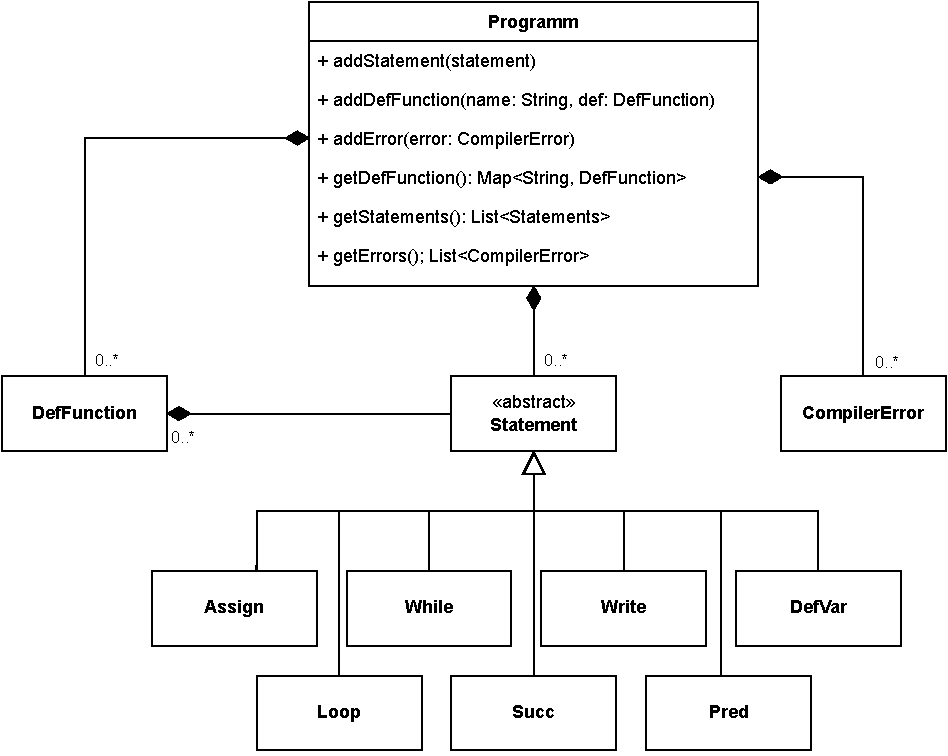
\includegraphics[width=13cm]{content/pictures/ClassDia.pdf}
	\caption{Ausschnitt der Datenstruktur}
	%	\source{\cite[S. 5]{SemtechCorporation.2020}}
	\label{pic:Semantic-Struct}
\end{figure}

\section{Durchlaufen des \acl{ast}}
Wie in \cref{subsec:antlr} bereits erklärt, wurde sich für diese Arbeit für den Visitor-Ansatz entschieden um den \ac{ast} zu durchlaufen. \ac{antlr} erzeugt beim Visitor-Ansatz eine \enquote{BaseVisitor}-Klasse. Diese beinhaltet für jeden Knoten eine Visit-Methode mit einem Parameter, welcher Informationen zum aktuellen Knoten enthält. Zusätzlich dazu ist die Methode in der Lage, einen beliebigen Datentyp zurückzugeben. In \cref{lst:parser-basevisitor} ist der Inhalt der BaseVisitor-Klasse zu sehen.

\begin{lstlisting}[language=java, caption=Inhalt der generierten BaseVisitor-Klasse, label={lst:parser-basevisitor}]
	public class WhileBaseVisitor<T> extends ... {
		@Override public T visitProg(ProgContext ctx) { return visitChildren(ctx); }
		@Override public T visitRead(ReadContext ctx) { return visitChildren(ctx); }
		...
	}
\end{lstlisting}

In dieser Arbeit wurde für jeden Knoten eine Visitor-Klasse erstellt, welche von der Visitor-Baseklasse erbt und die entsprechende Visit-Methode implementiert. Zusätzlich dazu hat jede Visitor-Klasse eine Referenz zum Programm, sodass auf bereits definierte Strukturen zugriffen oder eine Fehlermeldung hinzugefügt werden kann. Mithilfe der Informationen aus dem Parameter können mit einer dazugehörigen Visitor-Klasse wiederum die Unterknoten durchlaufenen werden, beispielsweise die Statements innerhalb eines Funktionsdefinitionsknotens. Jede Visit-Methode gibt zum Schluss eine Instanz der entsprechenden Datenstruktur zurück.

In \cref{lst:semantic-deffunction} ist exemplarisch dargestellt, wie die Visitorklasse für Funktionsdefinitionsknoten aufgebaut ist. Darin ist zu sehen, wie auf Unterknoten zugegriffen und zum Schluss ein Objekt zurückgegeben wird. Die Klasse \enquote{ProgramVisitor} nutzt die \enquote{DefFunctionVisitor}-Klasse, um DefFunction-Knoten zu durchlaufen und erhält bei Erfolg ein DefFunction Objekt zurück, welches die \enquote{Program}-Klasse in ihrer Collection speichern kann.

\begin{lstlisting}[language=java, caption=Prinzipieller Aufbau einer Visitorklasse, label={lst:semantic-deffunction}]
	public class DefFunctionVisitor extends WhileBaseVisitor<DefFunction> {
		
		private Program program;
		
		public DefFunctionVisitor(Program program) {
			this.program = program;
		}
		
		@Override
		public DefFunction visitDefFunction(DefFunctionContext ctx) {
			 // Greife auf den Knoten ID zu
			Token nodeId = ctx.ID().getSymbol();
			
			// Greife auf die Parameter zu
			List<TerminalNode> functionParameters = ctx.defParameters().ID();
			
			// Greife auf die Statements der Funktion zu
			List<StatementContext> functionStatements = ctx.statement(); 
			
			// Greife auf bereits existierende Funktionen zu
			Map<String,DefFunction> def = program.getDefFunctions();
			
			// Fuehre Pruefungen durch
			// ....
			// Fuege eine Fehlermeldung dem Programm hinzu 
			 // program.addError(...);
			
			// Durchlaufe die Statement Knoten
			AvailableVariables availableVariables = new AvailableVariables();
			StatementVisitor statementVisitor = new StatementVisitor(availableVariables, programm);
			
			for (var statement : functionStatements) {
				Statement stmt = statement.accept(statementVisitor);
				if (stmt != null) {
					statements.add(stmt);
				}
			}
			// Gebe bei Erfolg ein Objekt zurueck, welches die Funktion abbildet
			return new DefDunction(nodeId, parameters, statements)
		}
\end{lstlisting}

\section{Prüfungen}
Wie in \cref{lst:semantic-deffunction} zu sehen ist, werden innerhalb der Visitor-Klassen, das heißt während des durchlaufen des Baums, auch die eigentlichen semantischen Prüfungen durchgeführt. Dabei handelt es sich um eine Menge von (verschachtelten) If-Abfragen. Durch den Zugriff auf Unterknoten werden Informationen gewonnen, welche beispielsweise mit Informationen aus dem bisher geprüften Programm verglichen werden, um semantische Fehler zu finden. In \cref{lst:semantic-deffunction-mul} ist zu sehen, wie auf diese Weise bereits definierte Funktionen erkannt werden können. Mit einem ähnlichen Ansatz kann auch beispielsweise geprüft werden, ob bei einem Funktionsaufruf eine korrekte Menge von Parametern verwendet wurde. Es ist ebenfalls zu sehen, dass in einem Fehlerfall \enquote{null} zurück gegeben wird. Darauf muss die aufrufende Klasse achten und nur mit Objekten weiter arbeiten, welche nicht null sind.

\begin{lstlisting}[language=java, caption=Erkenne bereits definierte Funktionen, label={lst:semantic-deffunction-mul}]
	public class DefFunctionVisitor extends WhileBaseVisitor<DefFunction> {
		// ...
		@Override
		public DefFunction visitDefFunction(DefFunctionContext ctx) {
			// Greife auf den Knoten ID zu
			Token nodeId = ctx.ID().getSymbol();
			// ...
			// Greife auf bereits existierende Funktionen zu
			Map<String,DefFunction> def = program.getDefFunctions();
			
			// Ist eine Funktion mit selben Namen bereits definiert?
			if (def.get(nodeId.getText()) != null) {
				// Ja, fuege Progamm Fehler hinzu
				program.addError(...);
				return null;
			} else {
				// Nein
				return DefFunction(...);
			}
			// ...
		}
\end{lstlisting}

Die Prüfung, ob eine Variable, welche beispielsweise als Parameter verwendet werden soll, existiert, ist etwas komplexer. Das liegt daran, dass im Vergleich zu Funktionen kein globaler Namensraum existiert, in welchen alle Variablen eingetragen werden können. Stattdessen besitzt jede Funktion, jede Schleife und alle Variablen außerhalb einer Funktion einen eigenen Namensraum. Ein Beispiel dafür ist in \cref{lst:semantic-scope-expl} zu sehen.

\begin{lstlisting}[language=c, caption=Scope Beispiel, label={lst:semantic-scope-expl}]
var r0 := 5; // Erstelle Variable r0
var r1 := read(); // Erstelle Variable r1
loop(r1) begin: 
	// r1 und r0 existieren auch hier
	var s0 := r0; // Ist erlaubt
	// ... 
end
// r1 und r0 existieren immer noch
// s0 existiert nicht mehr
r0 := s0; // Ist ein semantischer Fehler
\end{lstlisting}

Um mit verschiedenen Namensräumen umzugehen, wurde eine neue Datenstruktur entworfen, welche in \cref{pic:Semantic-Scope} zu sehen ist. Eine Instanz dieser Datenstruktur wird jedem Statement-Visitor zusammen mit einer Referenz zum Programm mitgegeben. Herz der Datenstruktur sind zwei Stacks, welche jeweils ein String-Set beinhalten. In \enquote{availableVariables} werden alle verfügbaren Variablen gespeichert, während in \enquote{readOnlyVariables} ausschließlich Variablen landen, welche sich im Kopf einer Loop-Schleife befinden, da diese ausschließlich gelesen werden sollen.

\begin{figure}[h!]
	%\includegraphics[width=1\textwidth]{content/pictures/LoRaWAN-OSI.JPG}
	\centering
	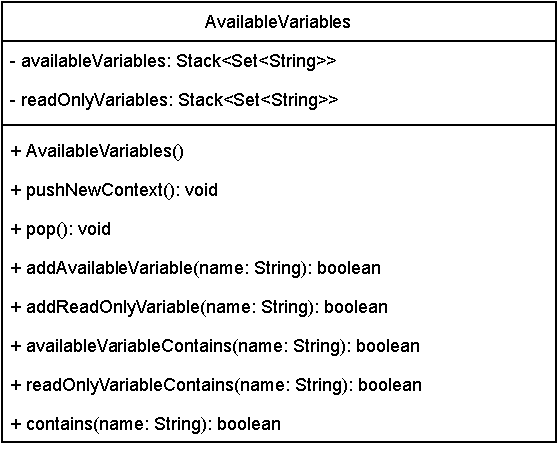
\includegraphics[width=9cm]{content/pictures/AvailableVar.pdf}
	\caption{Datenstruktur eines Namensraums}
	%	\source{\cite[S. 5]{SemtechCorporation.2020}}
	\label{pic:Semantic-Scope}
\end{figure}

Jedes Mal, wenn ein neuer Namensraums eröffnet wird, werden mit \enquote{pushNewContext} beide Sets in eine neue Schicht des Stacks kopiert und beim Verlassen des Namensraums mit \enquote{pop} wieder entfernt. Die \enquote{add}-, und \enquote{Contains}-Methoden arbeiten ausschließlich auf der obersten Schicht des Stacks, sodass nach einem \enquote{pop} alle hinzugefügten Variablen wieder verschwinden und der alte Stand wiederhergestellt ist. In \cref{lst:semantic-scope-loop} ist zu sehen, wie man mithilfe dieser Datenstruktur weitere Überprüfungen anstellen kann.

\begin{lstlisting}[language=java, caption=Umgang mit Namensräumen, label={lst:semantic-scope-loop}]
	public class LoopVisitor extends WhileBaseVisitor<Loop> {
		
		AvailableVariables availableVariables;
		Program program;
		
		public LoopVisitor(AvailableVariables availableVariables, Program program) {
			this.program = program;
			this.availableVariables = availableVariables;
		}
		
		@Override
		public Loop visitLoop(LoopContext ctx) {
			// Greife auf Knoten ID zu (Name der Variable im Schleifenkopf)
			Token varName = ctx.ID().getSymbol();
			// Pruefe ob Name ueberhaupt existiert
			if (availableVariables.contains(varName.getText())) {
				// Name existiert, pruefe ob Variable geschrieben werden darf
				if (!availableVariables.readOnlyVariablesContains(varName.getText())) {
					// Darf geschrieben werden, erzeuge einen neuen Namensraum
					availableVariables.pushNewContext();
					// Verbiete Schreiben der Variable im neuen Namensraum
					availableVariables.addReadOnlyVariable(varName.getText());
					// Durchlaufe alle Statements...
					// Schliese Namensraum
					availableVariables.pop();
					// Gib Loop zurueck
					return new Loop(...);
				} else {
					// Fuege Fehler hinzu...
				}
			} else {
				// Fuege Fehler hinzu 
				programm.addError(...)
				return null;
			}
		}
	}
\end{lstlisting}
